\chapter{Methodology}

% **************************** Define Graphics Path **************************
\ifpdf
	\graphicspath{{Chapter5/Figs/Raster/}{Chapter5/Figs/PDF/}{Chapter5/Figs/guided/}{Chapter5/Figs/unguided/}}
\else
    \graphicspath{{Chapter5/Figs/Vector/}{Chapter5/Figs/}}
\fi

\section{The OmpSs programming model}
\label{sec:ompss}
We choose to implement the new mechanisms proposed in this document in the OmpSs programming model.
The OmpSs programming model is a task-based programming model that offers a high level abstraction to the implementation of parallel applications for various homogeneous and heterogeneous architectures~\cite{OmpSs_PPL11,OmpSs}. It enables the annotation of code blocks or function declarations with the task directive, which declares a task. Every invocation of such a function creates a task that is executed concurrently with other tasks or parallel loops. OmpSs also supports task dependencies and dependency tracking mechanisms~\cite{StarSs}. 
OmpSs is composed of two main elements: the Mercurium compiler, responsible for the translation of the OmpSs annotation clauses to source code that calls to the Nanos++ API, and the Nanos++ runtime system, responsible for the internal creation and execution of the tasks. 
%OmpSs is built with the support of the Mercurium compiler, responsible for the translation of the OmpSs annotation clauses to source code, and the Nanos++ runtime system, responsible for the internal creation and execution of the tasks.

Nanos++ is an environment that serves as the runtime platform of OmpSs. It provides device support for heterogeneity and includes different plug-ins for implementations of schedulers, throttling policies, barriers, dependency tracking mechanisms, work-sharing and instrumentation. This design allows to maintain the runtime features by adding or removing plug-ins, facilitating the implementation of a new scheduler, or the support of a new architecture.

The implementations of the different scheduling policies in Nanos++ perform various actions on the states of the tasks. A task is \textit{created} if a call to this task is invoked but it is waiting until all its inputs are produced by previous tasks. When all the input dependencies are satisfied, the task becomes \textit{ready}. The ready tasks of the application at a given point in time are inserted in the \textit{ready queues} as stated by the scheduling policy. Ready queues can be thread-private or shared among threads. When a thread becomes idle, the scheduling policy picks a task from the ready queues for that thread to execute. The default OmpSs scheduler employs a \textit{breadth-first} policy~(BF)~\cite{Duran_schedulers_08} and implements a single first-in-first-out ready queue shared among all threads. When a task is ready, it is inserted in the tail of the ready queue and when a core becomes available, it retrieves a task from the head of the queue. BF does not differentiate among core types and assigns tasks in a first-come-first-served basis. We use this scheduler as our baseline.

The Nanos++ internal data structures support task prioritization. The task priority is an integer field inside the task descriptor that rates the importance of the task. If the scheduling policy supports priorities, the ready queues are implemented as \textit{priority queues}. In a priority queue, tasks are sorted in a decreasing order of their priority. The insertion in a priority queue is always ordered and the removal of a task is always from the head of the queue, i.e., the task with the highest priority. The priority of a task can be either set in user code, by using the \textit{priority} clause, which accepts an integer priority value or expression, or dynamically  by the scheduling policy, as is described in the next section.

Nanos++ runtime is the baseline of our runtime implementations.
We choose to implement our proposed scheduling policies within this runtime.
Also Nanos++ is easy to modify in order to reserve one thread responsible for the runtime.





\section{Evaluation}
\subsection{Evaluation platform}
\label{sec:platform}
The Hardkernel ODROID-XU3 development board has an 8-core Samsung Exynos 5422 chip with an ARM big.LITTLE architecture and 2GB of LPDDR3 RAM at 933MHz. The chip has four Cortex-A15 cores at 2.0GHz and four Cortex-A7 cores at 1.4GHz. The four Cortex-A15 cores form a \textit{cluster} with a shared 2MB L2 cache, and the Cortex-A7 share a 512KB L2 cache. The two \textit{clusters} are coherent, so a single shared memory application can run on both clusters, using up to eight cores simultaneously. In our experiments, we evaluate a set of possible combinations of fast and slow cores varying the total number of cores from two to eight. For the reminder of the paper, we refer to Cortex-A15 cores as \textit{big} and to Cortex-A7 cores as \textit{little}.

\subsection{Simulator}

To evaluate our approaches on larger multi-core systems we use the heterogeneous multi-core TaskSim simulator~\cite{AbstrLevels_TACO12}. 
TaskSim allows the specification of a heterogeneous system with two different types of cores: fast and slow. 
We can configure the amount of cores of each type and the difference in performance between the different types (performance ratio) in the TaskSim configuration file.
In our experiments, we will use up to a total of 80 distinct heterogeneous machine configurations.  
These comprise systems with the total number of cores ranging from 16 to 128, and the number of fast cores ranging from 1 to 16. 
For all these configurations, we evaluate the following performance ratios between fast and slow cores: 2$\times$, 2.5$\times$, 3$\times$, 3.5$\times$ and 4$\times$.

\subsection{Applications}
\label{sec:applications}
\begin{table*}[!t]
	\centering
	\scriptsize
	\caption{Evaluated benchmarks from the PARSEC benchmark suite}
	
	\setlength{\tabcolsep}{4pt}
	\begin{tabular}{|p{1.3cm}|p{7cm}|p{3cm}|p{1.6cm}|p{1cm}|}
	\hline
	\textbf{Benchmark} & \multicolumn{1}{|c|}{\textbf{Description}} & \multicolumn{1}{|c|}{\textbf{Input}} & \textbf{Parallelization} &\multicolumn{1}{|c|}{\textbf{Perf ratio}} \\
	\hline \hline
	blackscholes & Calculates the prices for a portfolio of European options analytically with the Black-Scholes partial differential equation. & 10,000,000 options & data-parallel &2.18 \\ \hline
	bodytrack & Computer vision application which tracks a 3D pose of a marker-less human body with multiple cameras through an image sequence. & 4 cameras, 261 frames, 4,000 particles, 5 annealing layers & pipeline & 4.16 \\ \hline
	canneal & Simulated cache-aware annealing to optimize routing cost of a chip design. & 2.5 million elements, 6,000 temperature steps & unstructured & 1.73 \\ \hline
	dedup & Compresses a data stream with a combination of global compression and local compression in order to achieve high compression ratios. & 351 MB data & pipeline & 2.67 \\ \hline
	facesim & Takes a model of a human face and a time sequence of muscle activation and computes a visually realistic animation of the modeled face. & 100 frames, 372,126 tetrahedra & data-parallel & 3.40 \\ \hline
	ferret & Content-based similarity search of feature-rich data (audio, images, video, 3D shapes, etc.) & 3,500 queries, 59,695 images database, find top 50 images & pipeline & 3.59 \\ \hline
	fluidanimate & Uses an extension of the Smoothed Particle Hydrodynamics method to simulate an incompressible fluid for interactive animation purposes. & 500 frames, 500,000 particles & data-parallel & 2.64 \\ \hline
	streamcluster & Solves the online clustering problem. & 200,000 points per block, 5 block & data-parallel & 3.48 \\ \hline
	swaptions & Intel RMS workload which uses the Heath-Jarrow-Morton (HJM) framework to price a portfolio of swaptions. & 128 swaptions, 1 million  simulations & data-parallel & 2.78 \\ \hline
	\end{tabular}
	\label{tab:parsec}
	\vspace{-0.3cm}
\end{table*}

In our experiments we use the PARSECSs benchmark suite~\cite{Chasapis:TACO2016}.
This benchmark suite offers a set of scientific real world applications implemented in OmpSs as well as pthreads. 
Table~\ref{tab:parsec} shows the applications and their characteristics.

Apart from the PARSECSs benchmark suite we use four scientific kernels implemented in the OmpSs programming model: Cholesky factorization, QR factorization, Heat diffusion and Integral Histogram. These benchmarks are accessible in the BSC Application Repository~\cite{BAR}. 

\textbf{Cholesky factorization} is a dense matrix operation that is used for solving linear equations in linear least square systems.
The OmpSs implementation of Cholesky blocks the input matrix into square blocks of floats and each task is responsible for performing the factorization on one block.

\textbf{QR Factorization} is a linear algebra algorithm that is used to solve the linear least squares problem \cite{QR}. 
We evaluate the performance of a blocked, communication avoiding QR implementation in OmpSs. 
We use an input blocked matrix of 8192$\times$8192 doubles forming 16$\times$16 blocks.

%\subsubsection{Heat Diffusion}
\textbf{Heat diffusion} uses the Gauss-Seidel method to compute the heat distribution on a matrix from \textit{x} heat sources. Heat diffusion implements an iterative solver of the equation that invokes the Gauss-Seidel method until the desired convergence is reached. We use a matrix of 8192$\times$8192 doubles and block size of 512$\times$512.

\textbf{Integral histogram} is a method to compute a cumulative histogram for each pixel of an image. 
The OmpSs implementation performs 
a horizontal and a vertical scan that transmit histograms to the blocks that reside on the right or below the current block.
Due to these transmissions, the application introduces many task dependencies. We use as input an image of 4096$\times$4096 pixels and block size of 512$\times$512.

\textbf{Blackscholes} from the PARSEC Benchmark Suite~\cite{Bienia:PhD2011}, is an Intel RMS benchmark. It calculates the prices for a portfolio of European options analytically with the Black-Scholes partial differential equation (PDE).
The OmpSs implementation~\cite{AbstrLevels_TACO12}, divides the work into units of a predefined block size. 
This block size allows having much more task instances than threads, which implies a much better load balance, as this is an embarrassingly parallel application with no dependencies among tasks in the same run.


\subsection{Metrics}
\label{sec:metrics}

All the experiments in this paper are performed on the Hardkernel Odroid XU3 described in Section~\ref{sec:platform}. In our experiments, we make use of the \texttt{cpufreq} driver to set the big cores to run at 1.6GHz and the little cores at 800MHz. 

\subsubsection{Performance}
To estimate the impact of the different kinds of cores, we evaluate seven configurations with different numbers of \textit{little} (L) and \textit{big} (B) cores, denoted \texttt{L+B}.
For each configuration and benchmark, we report the average performance of five executions taking into account only the parallel region of the application. Then, we report the speedup of the application over its serial execution time on one little core.
Equation~\ref{eq.speedup} shows the formula to compute the speedup.
\begingroup\makeatletter\def\f@size{9}\check@mathfonts
\begin{equation}
  \text{Speedup(L, B, method)} = \frac{\text{Exec. time(1, 0, serial)}}{\text{Exec. time(L, B, method)}}
\label{eq.speedup}
\end{equation}
\endgroup

\subsubsection{Power and Energy}
In this platform, there are four separated current sensors to measure in real time the power consumption of the cluster of A15 cores, the cluster of A7 cores, the GPU and DRAM. 
To gather the power and energy measurements, a background daemon is reading the machine power sensors periodically during the application execution with negligible overhead. Sensors are read every 0.27 seconds, and their values are written in a file. With the help of timestamps, we correlate the power measurements with the parallel region of the application in a  \emph{post-mortem} process. The reported power consumption is the average power that the SoC was consuming during five executions of each configuration, considering only the parallel region of the application. We then report the average power in Watts during the execution. 

Finally, in terms of energy and EDP, we report the total energy and EDP of the benchmark's region of interest normalized to the value that it consumes when running on four little cores with static threading.
Equations~\ref{eq.energy} and~\ref{eq.edp} show the formulas for these calculations.
\begingroup\makeatletter\def\f@size{8}\check@mathfonts
\begin{equation}
  \text{Normalized Energy(L, B, method)} = \frac{\text{Energy(L, B, method)}}{\text{Energy(4, 0, static-threading)}}
  \label{eq.energy}
\end{equation}
\begin{equation}
  \text{Normalized EDP(L, B, method)} = \frac{\text{EDP(L, B, method)}}{\text{EDP(4, 0, static-threading)}}
  \label{eq.edp}
\end{equation}
\endgroup

\subsection{Results}
\label{sec:results}

We have already made some progress in this thesis and have already covered some of the work to be done.
From our evaluation of the asymmetric system described in Section~\ref{sec:asymmetric} we found that adding little cores to a symmetric multi-core with big cores presents significant challenges for the application, OS and runtime developers. Little cores increase load imbalance and can degrade performance as a result. Relying on the application developer to deal with this asymmetry is complex and many applications are not ready. A dynamic OS scheduler such as \emph{GTS} can help in mitigating these problems, but the best results in terms of performance are obtained with the \emph{Task-based} approach. In terms of power and energy, the asymmetric multi-core provides significant benefits, although the symmetric multi-core with little cores remains the most energy-efficient configuration. The \emph{Task based} approach offers the highest performance with the lowest energy consumption when used on our 8-core system. With this in mind, the system-aware scheduling policies of a task-based programming model are meant to improve scheduling at the most appropriate level of the software stack.




\subsubsection{Evaluation of Scheduling Policies}
This section shows the results obtained from our scheduling policies described in Section~\ref{sec:scheduling}.
We compare our approaches against a dynamic implementation of the Heterogeneous Earliest Finish Time scheduler~\cite{HEFT} (dHEFT) in the OmpSs programming model.
The implementation assumes two different types of cores (big and
little) and keeps records of the tasks’ execution times in each core. The original HEFT~\cite{HEFT} implementation assumes the
prior knowledge of the TDG as well as the costs of the tasks.
In our case, since the evaluation consists of running real applications, the best way to compare HEFT to our proposal is
to keep the scheduling idea of HEFT and transform it from
a static to a dynamic scheduler. This means that dHEFT
discovers the costs of the tasks at runtime, computes a mean
value of the costs for each task-type and parameter-size duple for each type of core, and then finds the core that will
finish the task at the earliest possible time. 

To find the earliest possible executor, dHEFT maintains
one list per core (wlist) including the ready tasks waiting
to be executed by that core. When another task becomes
ready, dHEFT first checks if there are records of prior execution of this task. If the number of records is sufficient
(in our experiments we require a minimum of three records)
then the estimated execution time of the task is considered
stable. Then, using that estimated execution time, the task
is scheduled to the earliest executor by consulting the wlist
of all the cores. If the number of records is not sufficient
for one of the core types, then the task is scheduled to the
earliest executor of this core type to get another record of
that task-type and core-type execution time. In all cases,
dHEFT updates the history of records on every task execution to adapt for phase changes in the application.

We evaluate the applications Cholesky, QR, Heat diffusion, Integral Histogram and Bodytrack described in Section~\ref{sec:applications}.
To more precisely characterise the benchmarks, we plot the task cost variability for each benchmark on Figure~\ref{distributions}.
For each of these plots, the $x$ axis shows the normalized task cost and the $y$ axis the number of tasks that correspond to this task cost (e.g. how many tasks have this cost).
This is used to show how heterogeneous each application is and explain the behaviour of the heterogeneous schedulers that take into account the execution time.

Figure~\ref{speedup} shows the speedup obtained for each application,  scheduler and machine set-up.
The x axis shows for each application the total number of cores at the bottom and the number of big cores at the top.
We classify the benchmarks according to their task cost variability to easier explain the results.

%------ HEAT ---------- very low variability


Heat diffusion is the kernel with the lowest task variability (e.g. the most homogeneous benchmark) as shown in Figure~\ref{heat_dist}.
CATS, HYBRID and dHEFT increase the performance of heat by 10\% on 8 cores and obtain similar results for the other numbers of cores by rearranging the tasks according to the type of the resources.
Due to its high per-task overheads and the homogeneity of the benchmark, CPATH scheduler cannot outperform the random BF scheduler. 
Moreover, for this benchmark, CPATH detects only 23\% of the tasks to be critical while CATS and HYBRID detect approximately 54\%, when running on 8 cores.
This happens because with CPATH, it is more likely to have zero-priority tasks during the task submission step, due to the post-exit task priority assignment that the algorithm introduces. 
The zero-priority tasks are considered non-critical and this limits the utilization of the big cores with CPATH. 

%---------- CHOLESKY 16x16 ------------ low variability

Cholesky 16$\times$16 has also low task cost variability. 
The improvements of CATS, dHEFT and HYBRID over BF are limited to around 7\% when running on 8 cores.
These schedulers perform almost the same for the rest numbers of cores and CPATH performs almost the same as BF. 
The increased overheads of CPATH do not pay off with better schedules since, for the same reason as in the case of Heat diffusion, only 10\% of the tasks are marked as critical on 8 cores (while 21\% CATS and 16\% HYBRID).

%--------- BODYTRACK --------------- low variability - very high number of tasks

Bodytrack shows low task cost variability, since 99\% of its tasks have similar execution times.
In this case, contrarily to the previous benchmarks CPATH manages to achieve similar speedups to CATS and HYBRID and outperform BF by up to 15\%.
This is due to the very high number of tasks of bodytrack; CPATH overcomes its overheads by using the detected task execution times for a higher number of tasks.
In other words, the learning phase of CPATH becomes a smaller proportion of the total execution of the benchmark.
Since bodytrack has so many tasks, the per-task overhead of CPATH is around 120us while for CATS it is 93us.
On the other hand, dHEFT shows poor performance because of the overheads of analyzing a TDG with a high number of tasks to compute the earliest finish time schedule.

%---------- HISTOGRAM --------------- medium variability - good amount of tasks (2048)

Integral histogram is characterized by medium task cost variability and high amount of tasks.
This benchmark is dependency intensive with limited parallelism, which makes scheduling decisions very important.
CATS and HYBRID schedulers achieve the best results since they focus more on the TDG structure and dependencies, improving BF by 30\% and 27\% respectively.
CPATH and dHEFT are slightly less efficient and improve BF by 19 and 21\% respectively.

%---------- CHOLESKY 8x8 -------------- high variability but very few tasks

For Cholesky 8$\times$8, the heterogeneous schedulers CATS, HYBRID and dHEFT constantly improve the performance of BF and reach up to 45\% improvement on 8 cores.
It is observed here that dHEFT indeed performs better when the number of tasks is limited as this workload has 120 tasks in total.
The additional overheads of CPATH do not compensate with increased performance in this case because there are not enough tasks to apply the better scheduling.

%---------------- QR ------------ the highest variability and good number of tasks (1496)

QR factorization is the highest task cost variability benchmark as shown in Figure~\ref{qr_dist}.
This is the reason why HYBRID gradually outperforms CATS as we increase the number of cores.
%With a small additional overhead,
%(CATS: 1419us while HYBRID: 14514us per-task overhead)
%as Table~\ref{tab.apps} shows, 
HYBRID manages to efficiently detect critical tasks that reside on the critical path and boost their execution reaching 17\% improvement over the baseline.
For this benchmark, CPATH also reaches a 13\% improvement over BF since task cost matters in this case. 
However, CPATH speedup is still limited compared to HYBRID because of the higher scheduling overheads which in this case is 1.8$\times$ higher than CATS overheads.
dHEFT also improves BF by finding the earliest executor of each task, but the improvement is limited to 11\% which is lower than the other approaches.

%--------- SUMMARY ---------------

This section showed a straight comparison between different heterogeneous schedulers.
It is important to note that schedulers like CPATH and HYBRID, that detect the time-based critical path, are the best choices when the application has a large amount of tasks.
This is because the additional overheads of these schedulers for critical path computation take place only when there are new tasks on the TDG or when there is a task exit of an untracked task type. 
When the TDG has been completely created, and as soon as the cost of every task type of the application has been tracked, the schedules of these approaches are purely beneficial.
On the other hand, schedulers like dHEFT perform the same steps for every single task that becomes ready, affecting the entire execution since the exit of a task triggers the execution of its successors that become ready. 
Thus, as the number of tasks is increased, the additional scheduling overheads are increased when using dHEFT-like approaches.
CATS scheduler is an efficient scheduling solution for any number of tasks and task cost distributions.
The additional CATS overheads take place only during task creation and are smaller than CPATH overheads with the drawback of not considering the task execution time.
If we have to choose the best and most generic heterogeneous scheduling approach among the presented schedulers the HYBRID scheduler is the best choice, since it computes an accurate critical path only

\begin{figure*}[!t]
\centering
\begin{subfigure}[b]{0.3\textwidth}
  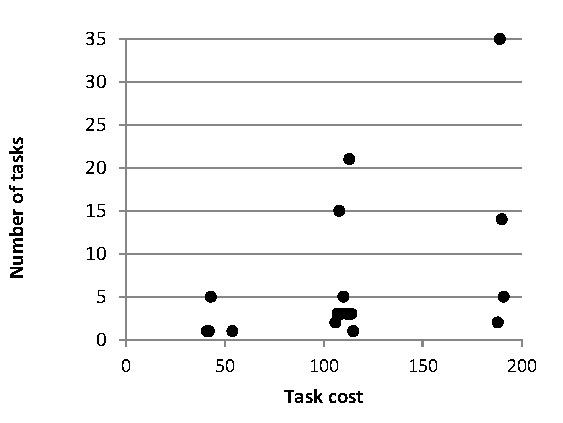
\includegraphics[width=\textwidth]{Figs/cholesky_8x8_distribution.pdf}
  \caption{Cholesky 8$\times$8}
  \label{cholesky8x8_dist}
\end{subfigure}
\begin{subfigure}[b]{0.3\textwidth}
  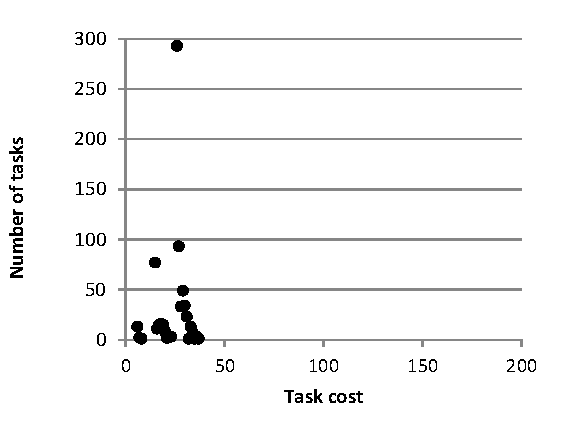
\includegraphics[width=\textwidth]{Figs/cholesky_16x16_distribution.pdf}
  \caption{Cholesky 16$\times$16}
  \label{cholesky16x16_dist}
\end{subfigure}
\begin{subfigure}[b]{0.3\textwidth}
  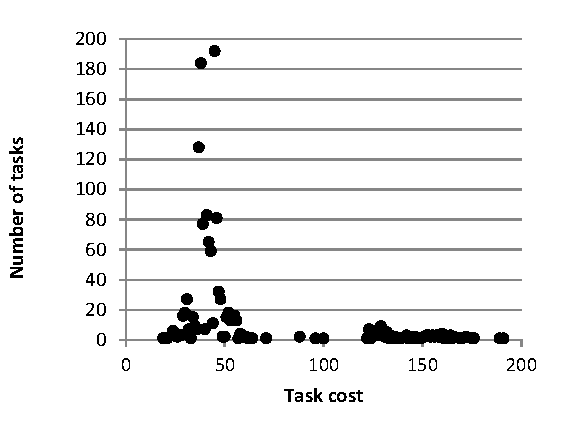
\includegraphics[width=\textwidth]{Figs/QR_16x16_distribution.pdf}
  \caption{QR factorization}
  \label{qr_dist}
\end{subfigure}
\begin{subfigure}[b]{0.3\textwidth}
  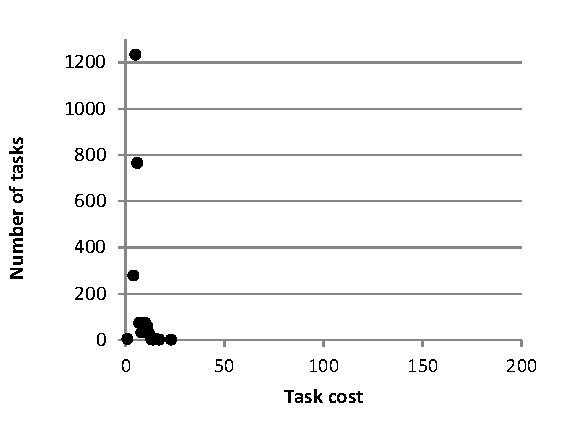
\includegraphics[width=\textwidth]{Figs/heat_16x16_distribution.pdf}
  \caption{Heat diffusion}
  \label{heat_dist}
\end{subfigure}
\begin{subfigure}[b]{0.3\textwidth}
  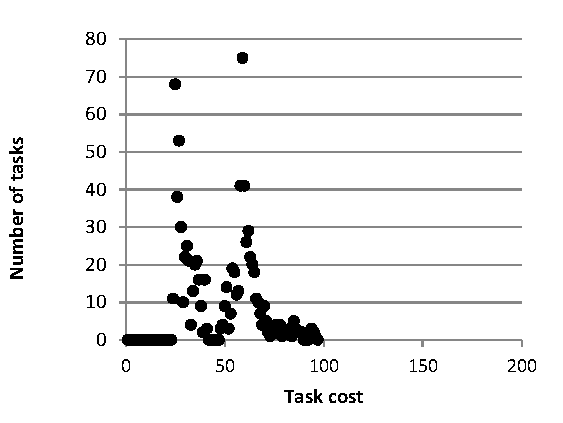
\includegraphics[width=\textwidth]{Figs/histogram_8x8_distribution.pdf}
  \caption{Integral Histogram}
  \label{histogram_dist}
\end{subfigure}
\begin{subfigure}[b]{0.3\textwidth}
  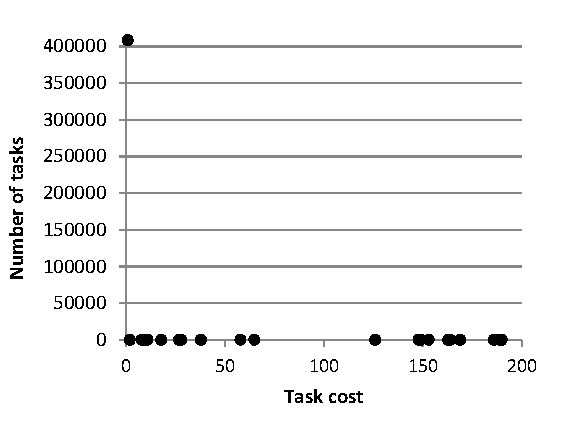
\includegraphics[width=\textwidth]{Figs/bodytrack_native_distribution.pdf}
  \caption{Bodytrack}
  \label{bodytrack_dist}
\end{subfigure}
  \caption{Task cost distribution for each application. Results are based on 4BIG-core executions. $x$ axis shows the cost of the tasks and $y$ axis shows the number of tasks with the corresponding task cost.}
  \label{distributions}
  \vspace{-0.4cm}
\end{figure*}


\begin{figure*}[!t]
  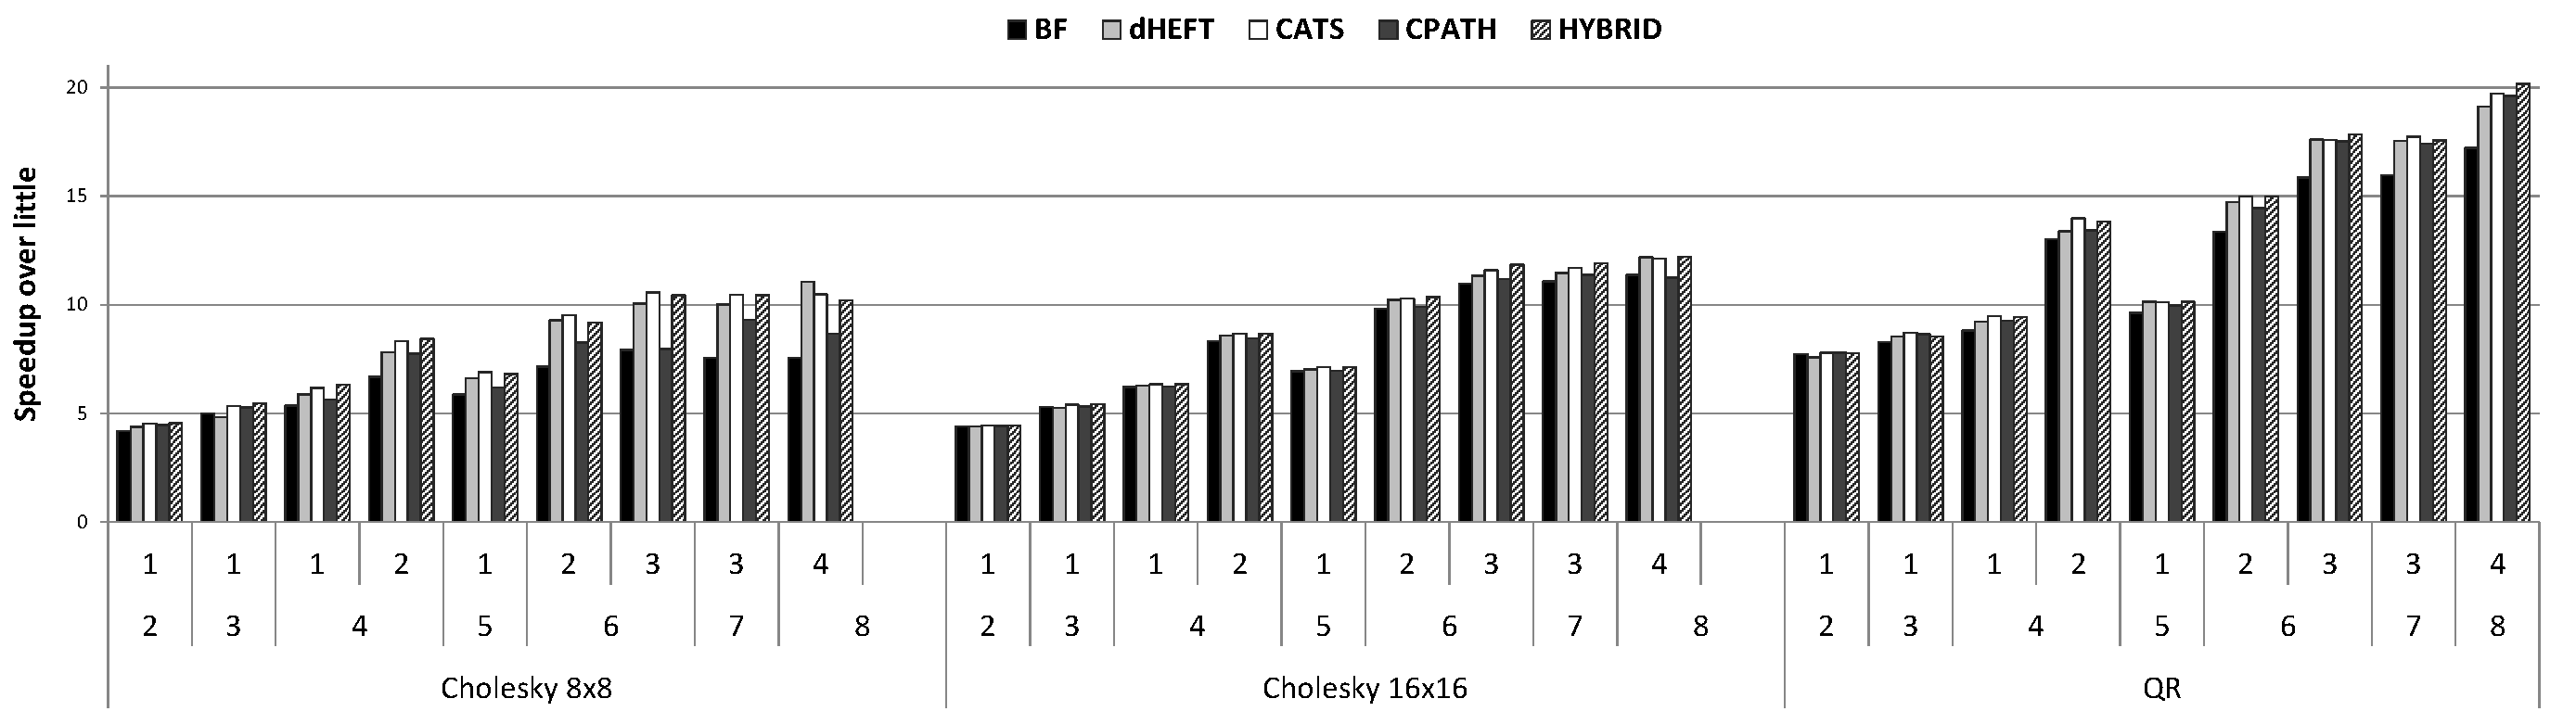
\includegraphics[width=\textwidth]{Figs/speedup_apps1.pdf}
   \vspace{-0.4cm}

  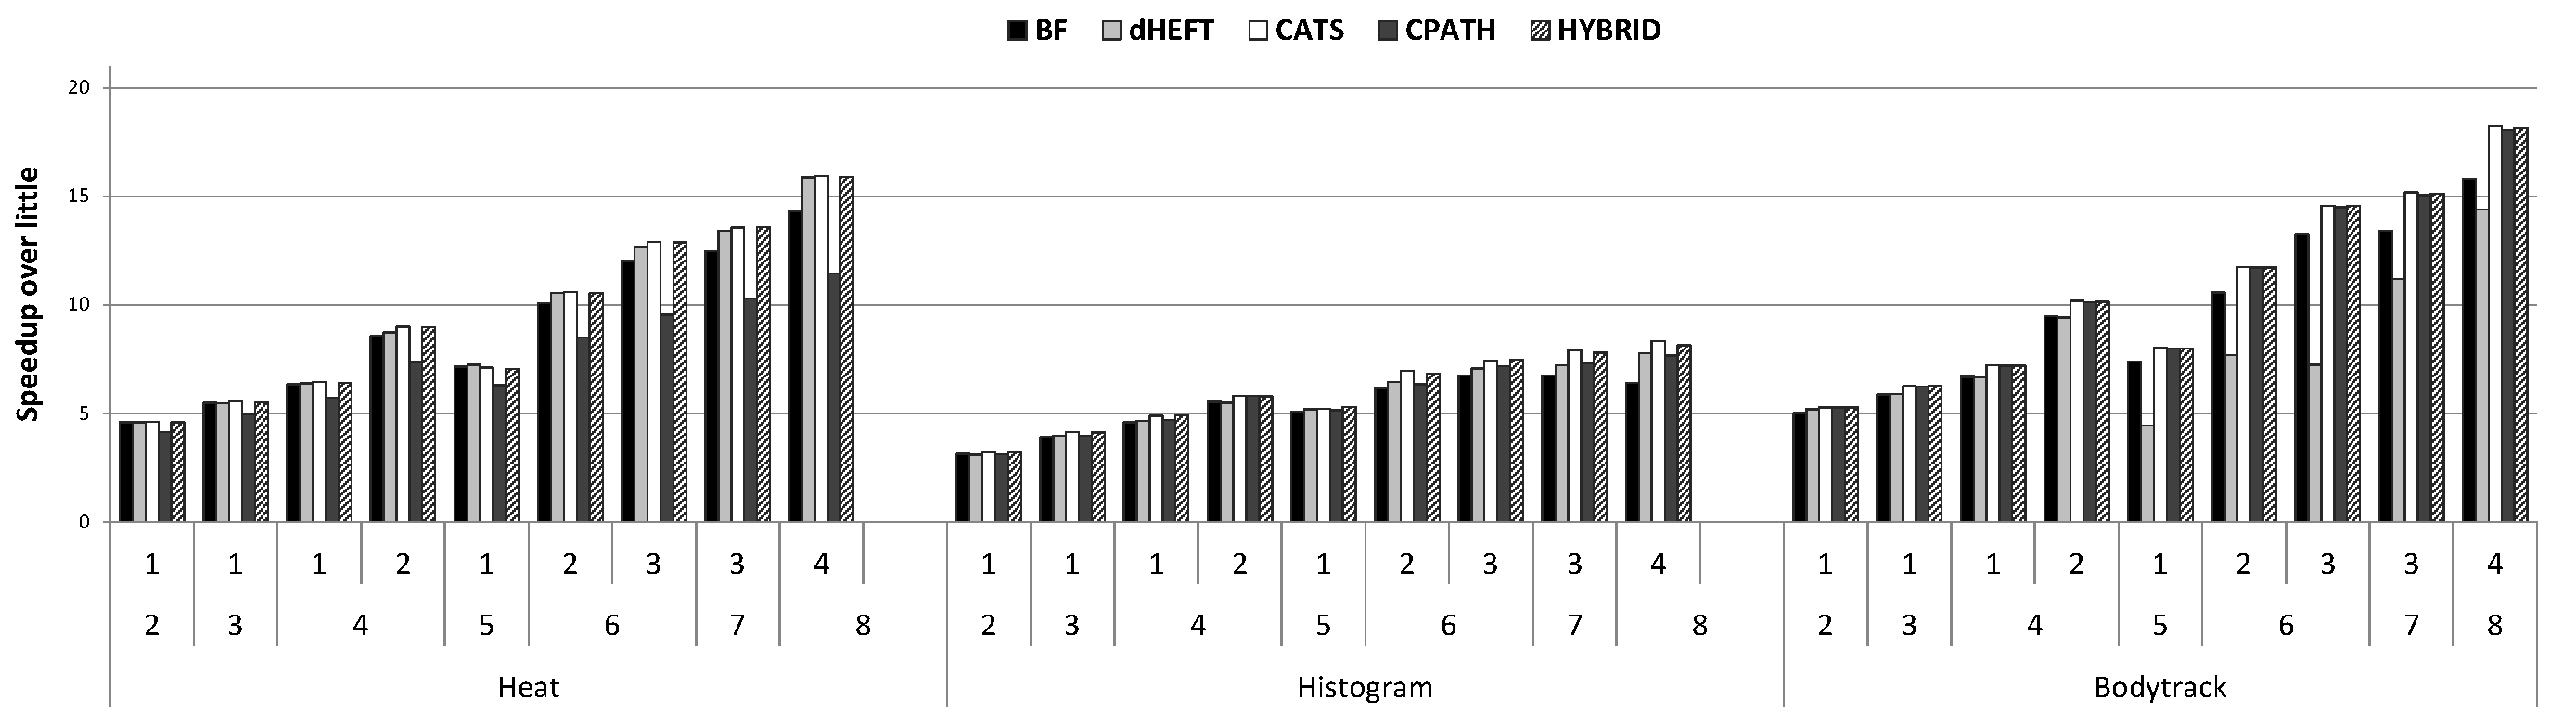
\includegraphics[width=\textwidth]{Figs/speedup_apps2.pdf}
  \caption{Speedups obtained for each scheduler and each application}
  \label{speedup}
  \vspace{-0.4cm}
\end{figure*}  

\subsubsection{Evaluation of Runtime Activity Manager}
In our preliminary evaluation of three workloads using RAM we observe very promising results.
Specifically, Figure~\ref{speedupRAM} shows the speedup of the baseline and RAM approach when we simulate the applications on up to 512 cores.
We can see that for the baseline runtime, performance saturates as we increase the number of cores. 
This happens due to the task creation overhead, which we overcome by accelerating it on the special hardware. 

\begin{figure*}[!t]
  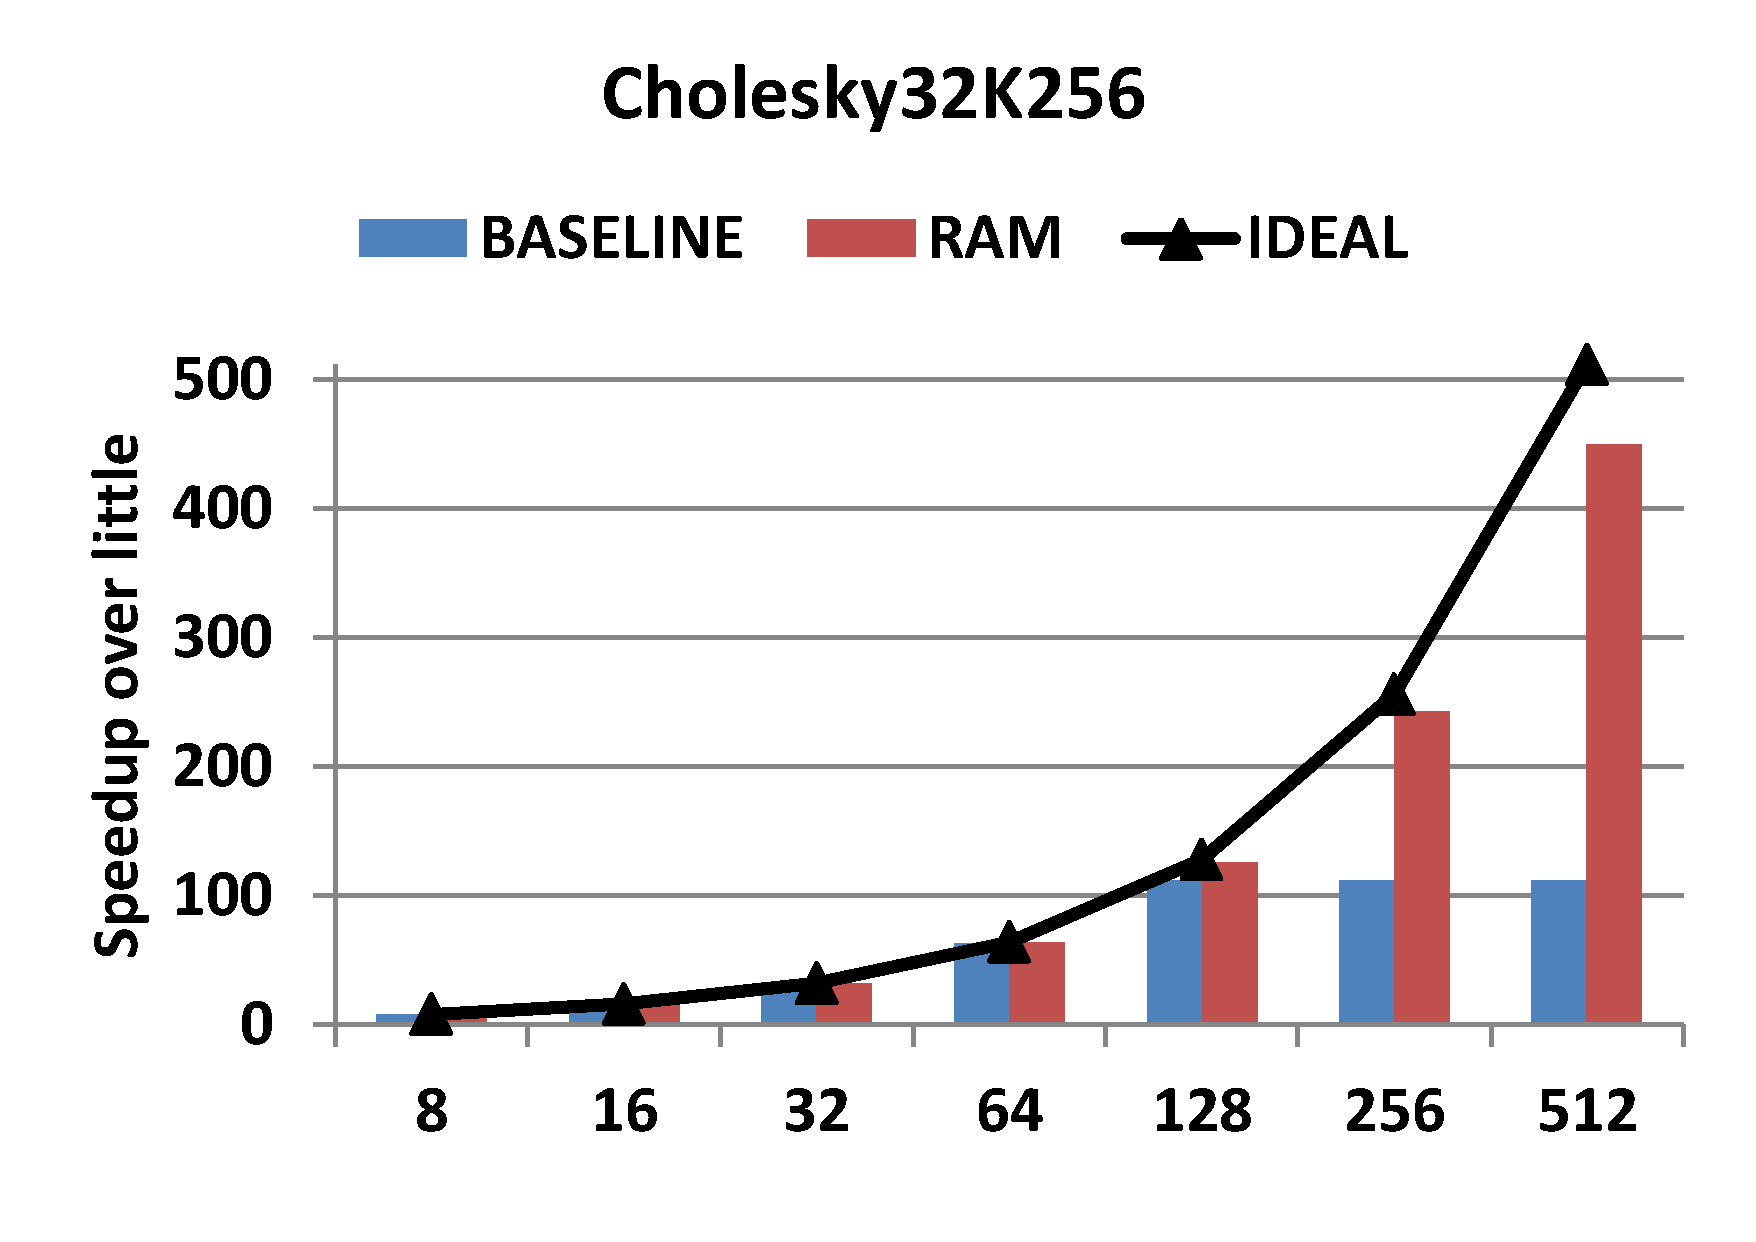
\includegraphics[width=0.32\textwidth]{Figs/cholesky_32K256.pdf}
  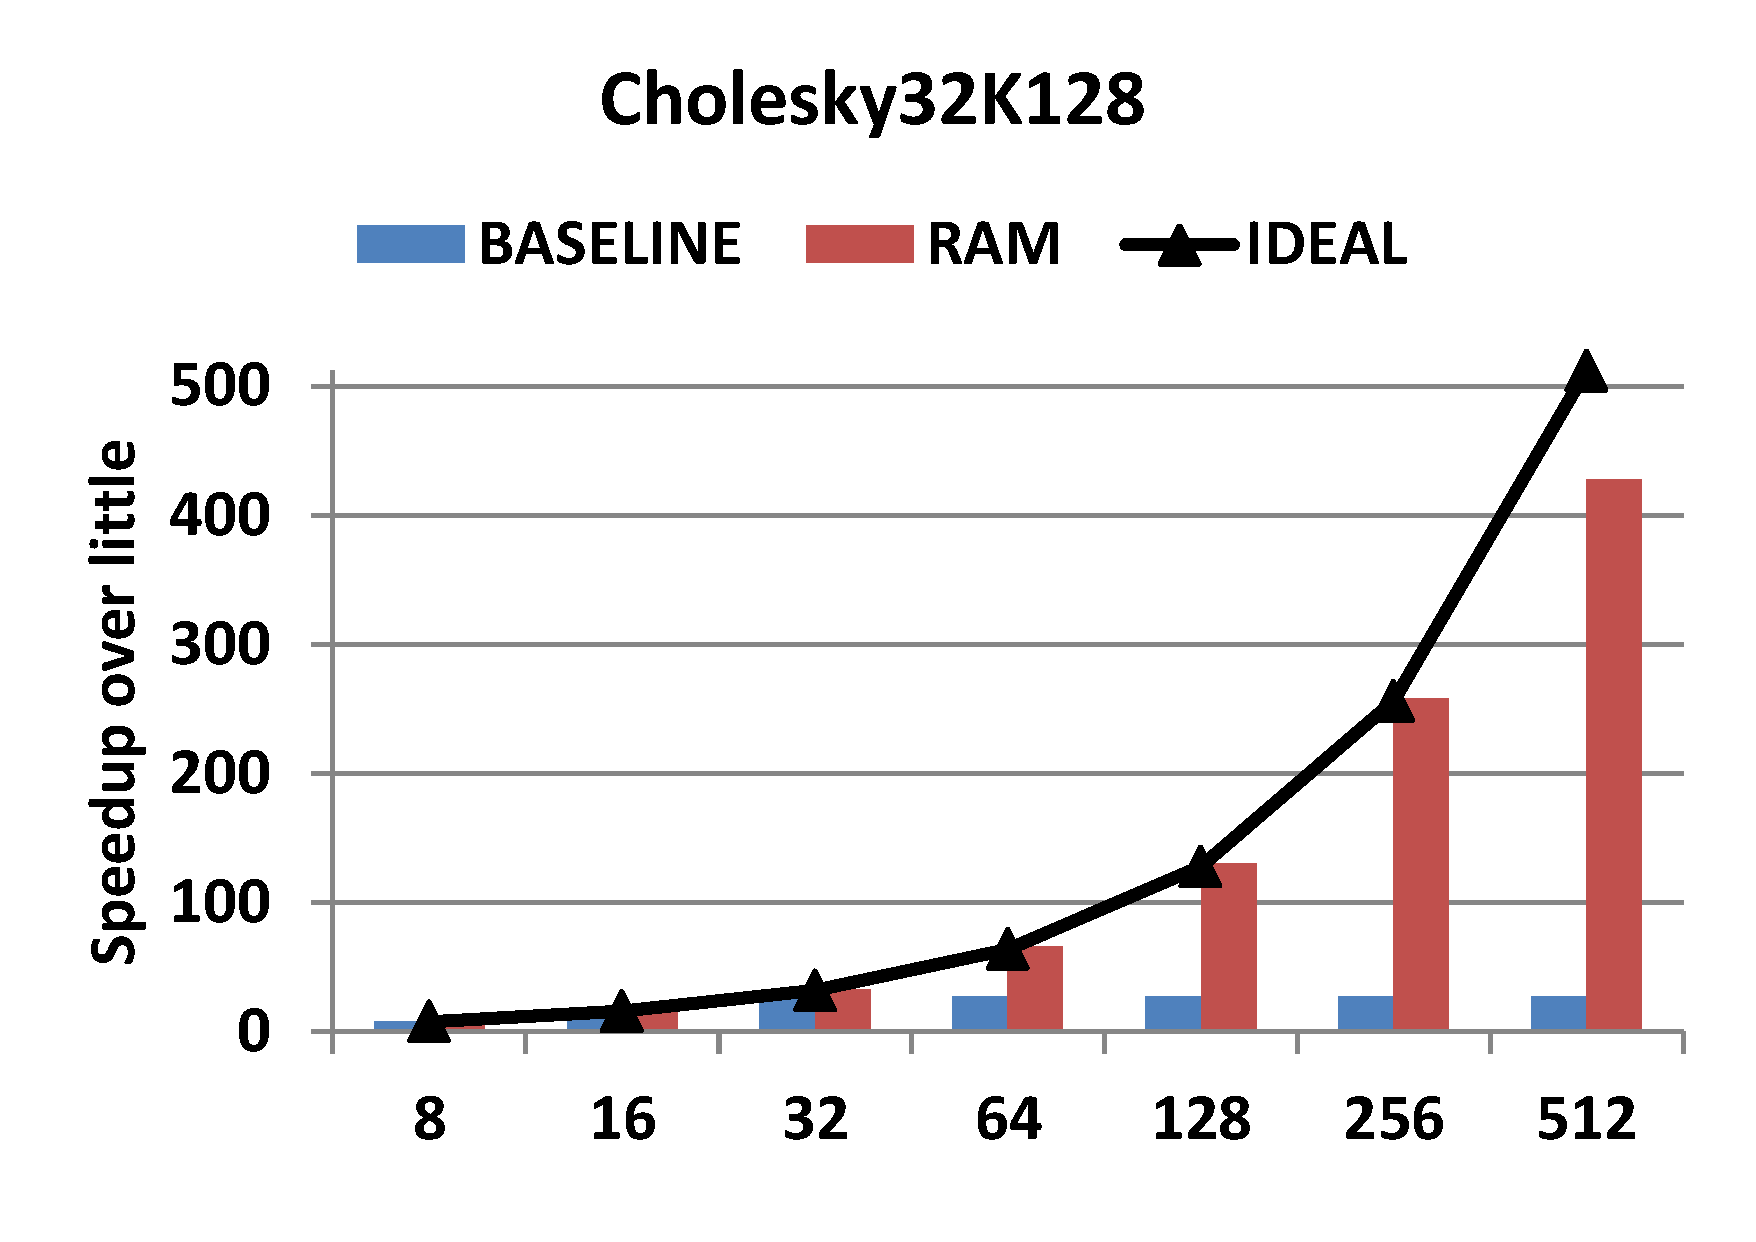
\includegraphics[width=0.32\textwidth]{Figs/cholesky_32K128.pdf}
  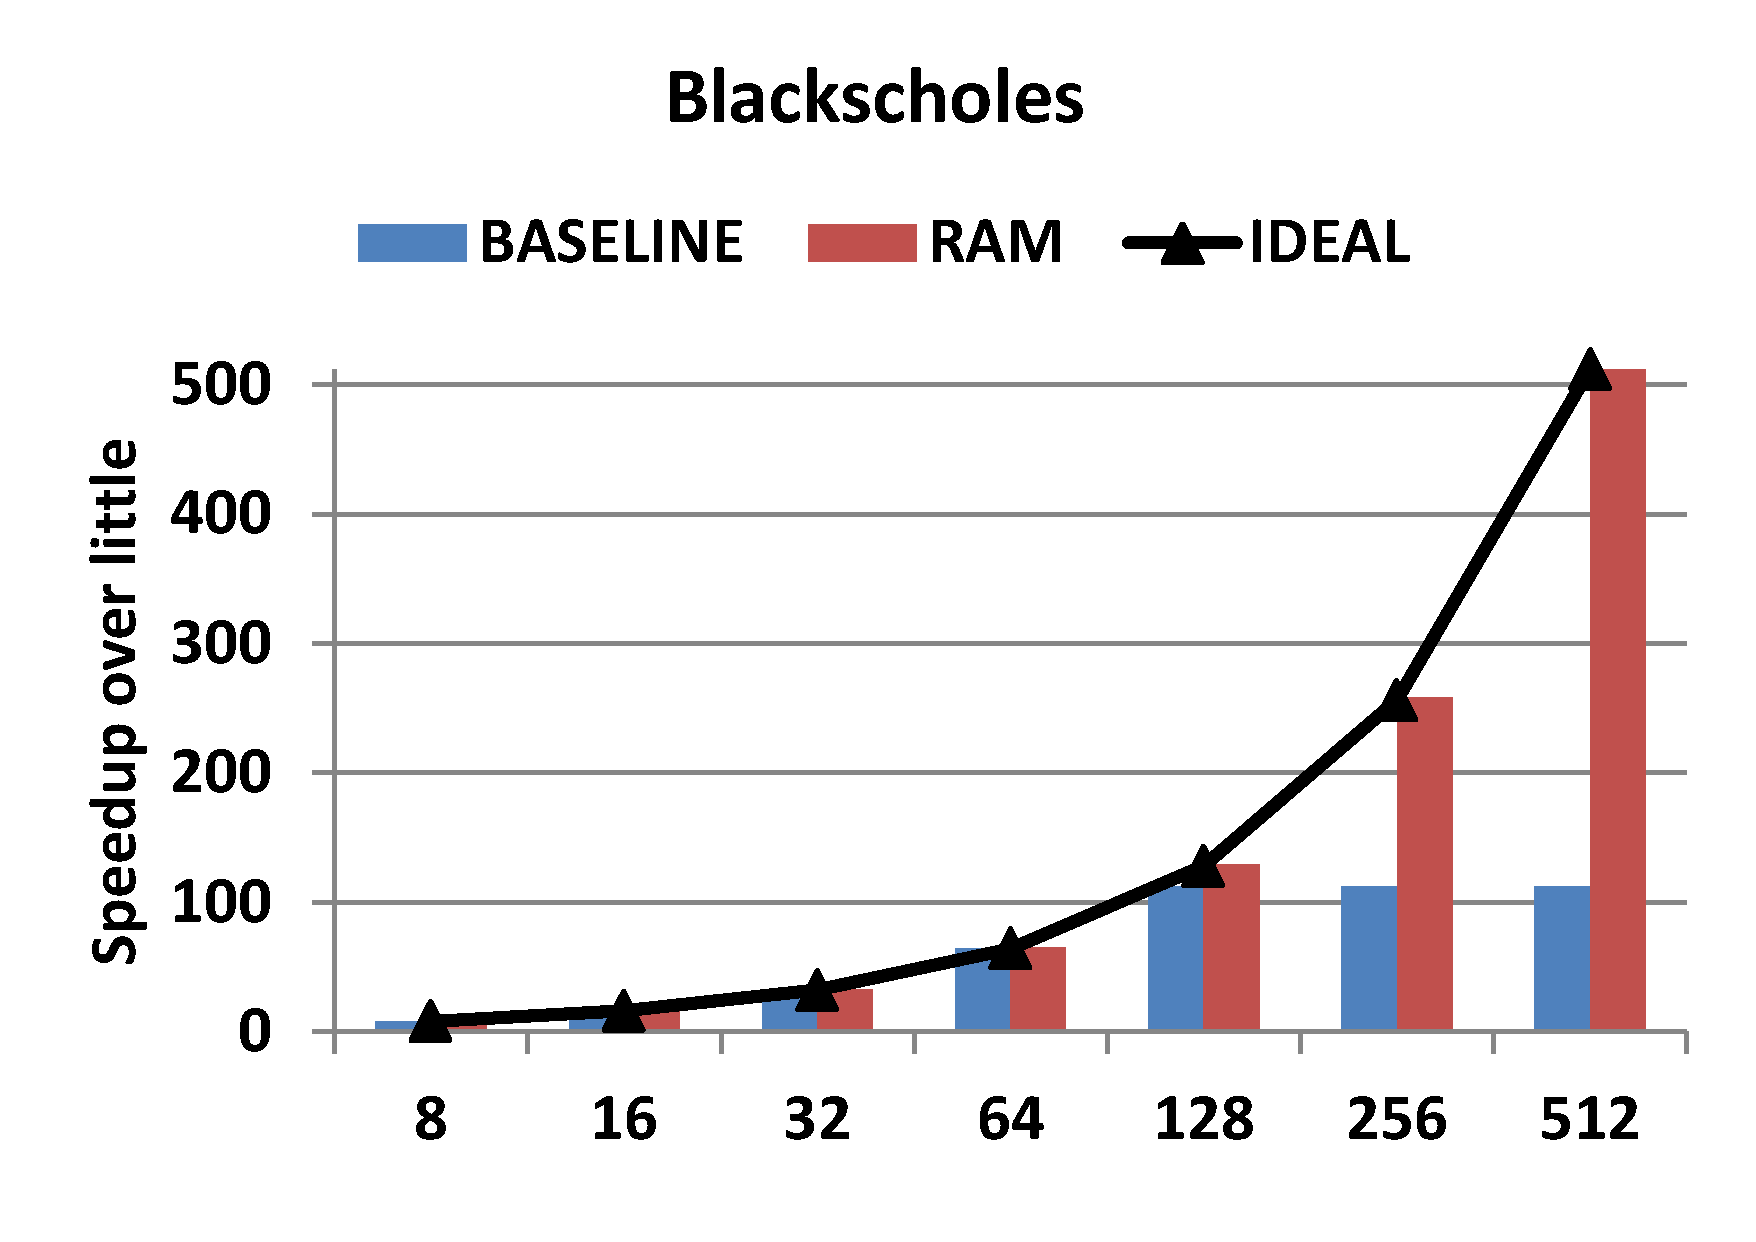
\includegraphics[width=0.32\textwidth]{Figs/blackscholes.pdf}
  \caption{Speedups obtained for default OmpSs runtime (BASELINE) and RAM for each application}
  \label{speedupRAM}
\end{figure*}  

We plan to further improve this evaluation by adding results for asymmetric systems.
